\section*{1. Time Conditioning Comparison (EC1)}

\subsection*{Problem \& Approach}
The \textbf{main HW3 baseline} uses an unconditioned EmojiViT: the network receives only $z_t$ with no explicit timestep, relying on $\|z_t\|$ to encode $t$ at $D = 3072$ (Sahraee-Ardakan et al., 2026). EC1 asks whether adding explicit time conditioning improves on that baseline. We train a FiLM/adaLN variant (\texttt{EmojiViTFiLM}) alongside a re-trained copy of the main HW3 configuration (``no-time baseline'') for 300 epochs with identical optimizer settings.

\subsection*{Results}

\begin{table}[h]
\centering
\begin{tabular}{l c c c c}
\toprule
\textbf{Model} & \textbf{Final Train Loss} & \textbf{Final Val Loss} & \textbf{Params} & \textbf{Relation to Main HW3} \\
\midrule
Main HW3 (500 ep.) & 0.1531 & 0.1857 & 4,841,920 & submitted baseline \\
Main HW3 (300 ep.) & 0.1747 & 0.1908 & 4,841,920 & same checkpoint as EC \\
No-time (EC re-train) & 0.1753 & 0.1910 & 4,841,920 & reproduces main HW3 setup \\
FiLM time-conditioned & 0.1518 & 0.1810 & 7,335,872 & EC addition \\
\bottomrule
\end{tabular}
\caption{EC1 vs.\ main HW3. The no-time EC model matches main HW3 at epoch 300; FiLM beats both at 300 epochs but has not yet matched main HW3's 500-epoch val loss (0.1857).}
\label{tab:ec1_loss}
\end{table}

\begin{figure}[h]
    \centering
    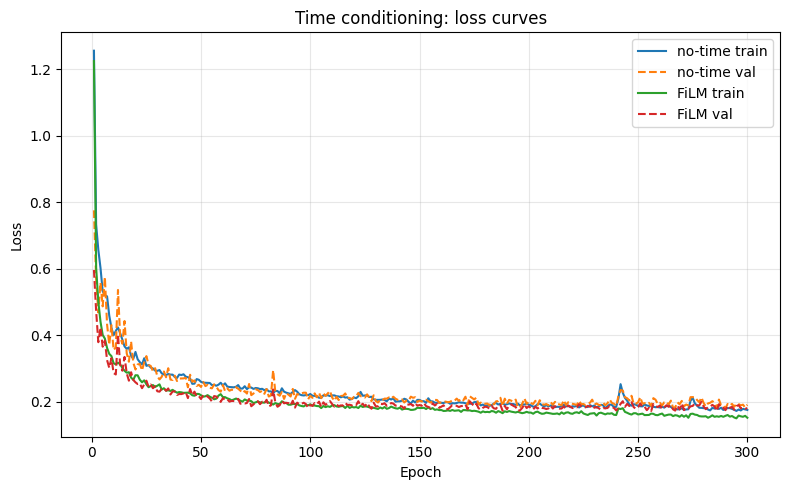
\includegraphics[width=0.75\textwidth]{figures/ec1_loss.png}
    \caption{Train and validation loss: no-time (main HW3 config) vs.\ FiLM.}
    \label{fig:ec1_loss}
\end{figure}

\begin{figure}[h]
    \centering
    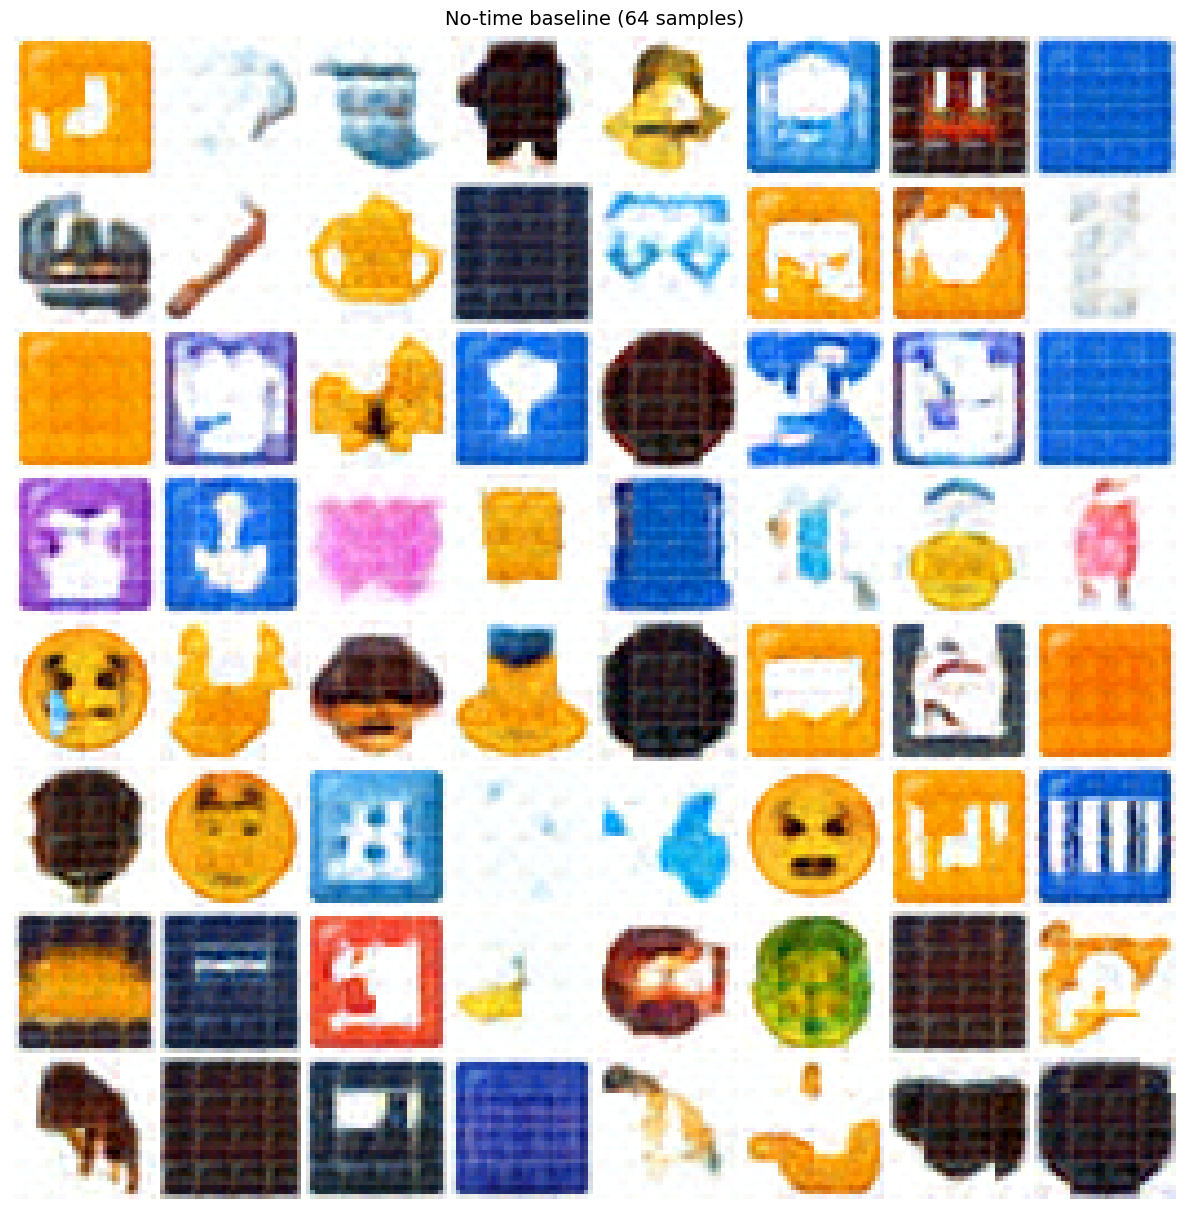
\includegraphics[width=0.48\textwidth]{figures/ec1_samples_no_time.png}
    \hfill
    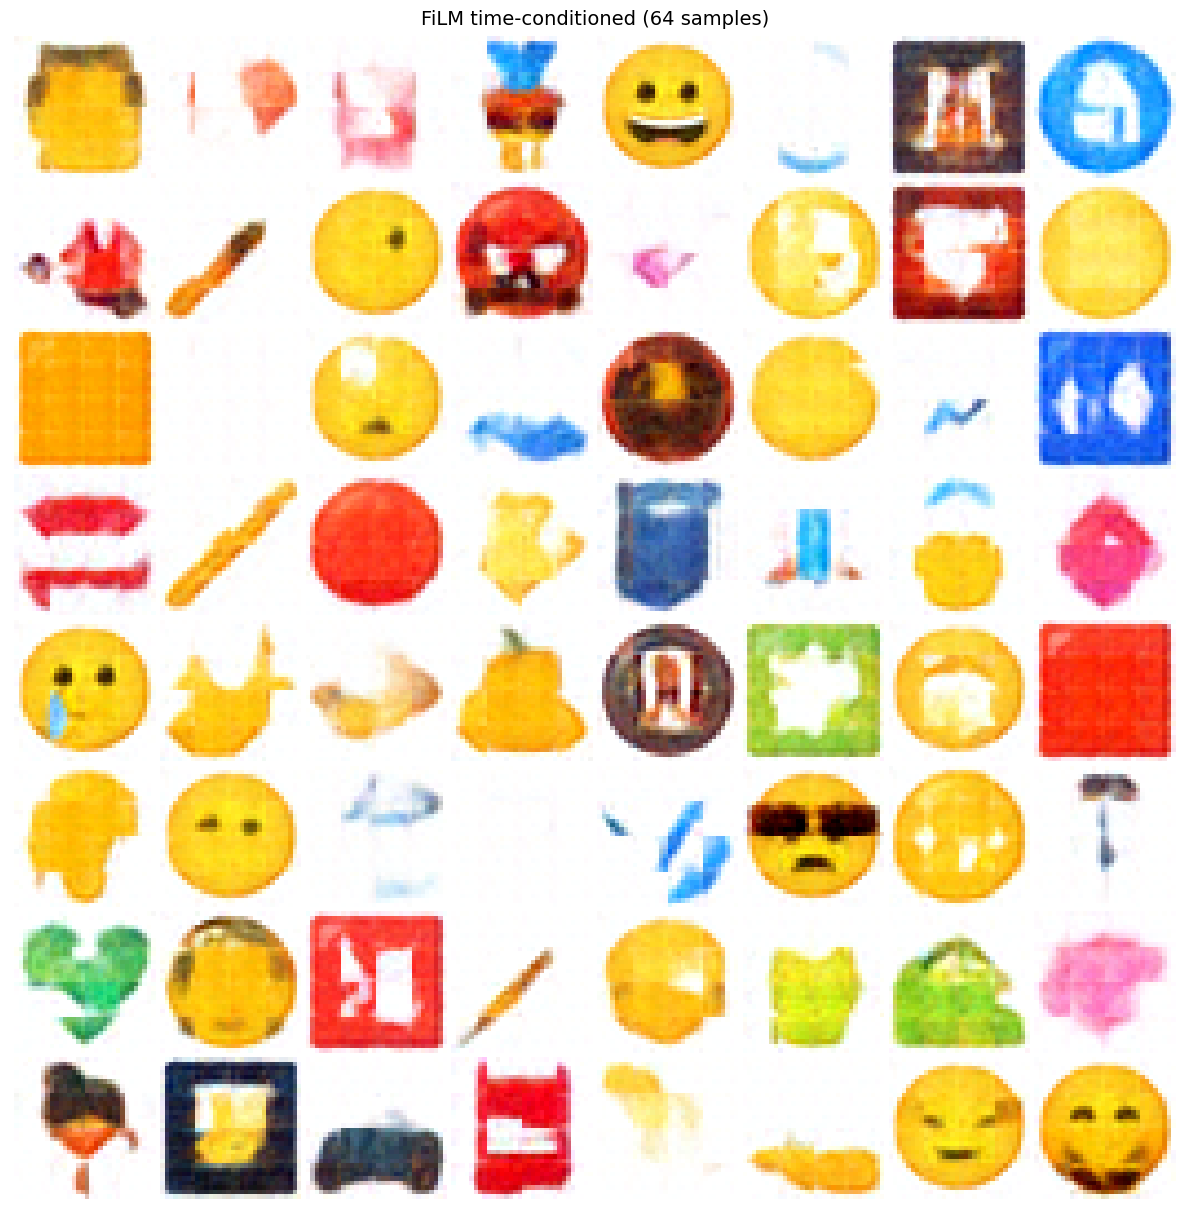
\includegraphics[width=0.48\textwidth]{figures/ec1_samples_film.png}
    \caption{Left: EC no-time samples (same config as main HW3). Right: FiLM samples (same noise). Compare to Figure~\ref{fig:main_samples}.}
    \label{fig:ec1_samples}
\end{figure}

\begin{figure}[h]
    \centering
    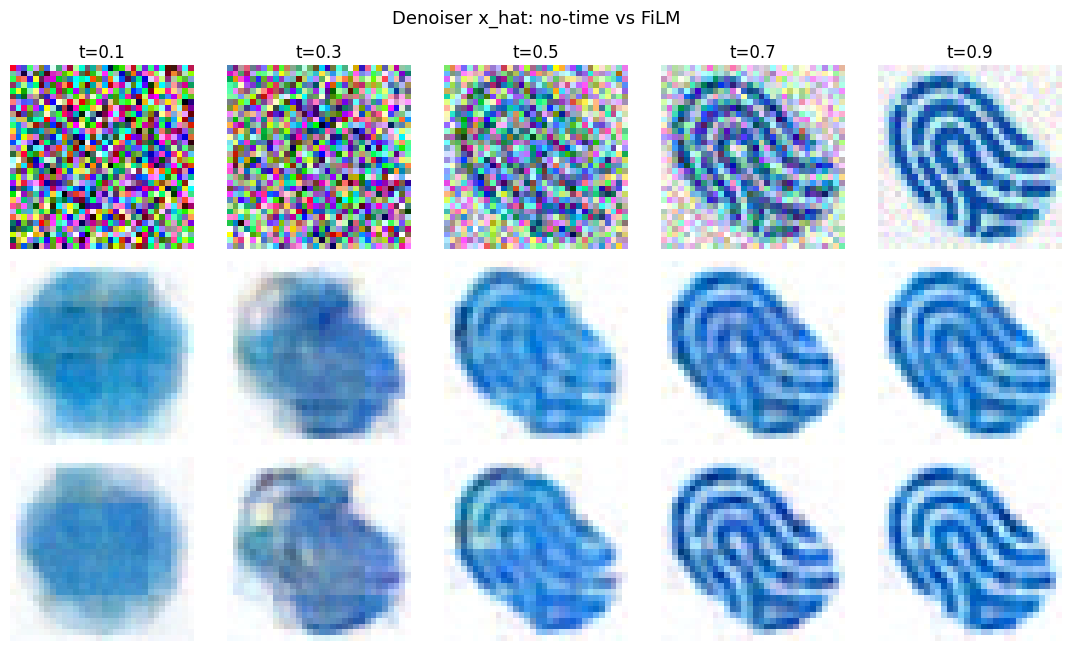
\includegraphics[width=0.85\textwidth]{figures/ec1_denoiser.png}
    \caption{Denoiser $\hat{x}$ at $t \in \{0.1, \ldots, 0.9\}$: noisy $z_t$ (top), no-time / main HW3 config (middle), FiLM (bottom).}
    \label{fig:ec1_denoiser}
\end{figure}

\subsection*{Discussion}
Relative to main HW3, explicit time conditioning yields a modest val-loss improvement at 300 epochs (0.1910 $\to$ 0.1810) at +51\% parameters. FiLM has lower \emph{train} loss at 300 epochs than main HW3 achieves even at 500 (0.1518 vs.\ 0.1531), but its val loss (0.1810) has not yet beaten main HW3's fully trained val (0.1857)---likely because EC1 stopped early. Sample grids are comparable to main HW3 (Figure~\ref{fig:main_samples}); FiLM appears slightly sharper in places. Overall, the gain is modest, consistent with ``Geometry of Noise'': at this dimensionality, main HW3's unconditioned design already captures most of what time conditioning provides.
